% !TEX TS-program = pdflatex
% !TEX encoding = UTF-8 Unicode

% This is a simple template for a LaTeX document using the "article" class.
% See "book", "report", "letter" for other types of document.

\documentclass[12pt]{article} % use larger type; default would be 10pt

\usepackage[utf8]{inputenc} % set input encoding (not needed with XeLaTeX)

%% Examples of Article customizations
% These packages are optional, depending whether you want the features they provide.
% See the LaTeX Companion or other references for full information.

%% PAGE DIMENSIONS
\usepackage{geometry} % to change the page dimensions
%\geometry{letterpaper} % or letterpaper (US) or a5paper or....
 \geometry{margin=1.5in} % for example, change the margins to 2 inches all round
% \geometry{landscape} % set up the page for landscape
%   read geometry.pdf for detailed page layout information

\usepackage{graphicx} % support the \includegraphics command and options

% \usepackage[parfill]{parskip} % Activate to begin paragraphs with an empty line rather than an indent

%% PACKAGES
\usepackage{listings}
\usepackage{booktabs} % for much better looking tables
\usepackage{array} % for better arrays (eg matrices) in maths
\usepackage{paralist} % very flexible & customisable lists (eg. enumerate/itemize, etc.)
\usepackage{verbatim} % adds environment for commenting out blocks of text & for better verbatim
%\usepackage{subfig} % make it possible to include more than one captioned figure/table in a single float
% These packages are all incorporated in the memoir class to one degree or another...
\usepackage[usenames,dvipsnames]{color}
\usepackage{caption}
\usepackage{subcaption}
\usepackage{float}
%% HEADERS & FOOTERS
\usepackage{fancyhdr} % This should be set AFTER setting up the page geometry
\pagestyle{fancy} % options: empty , plain , fancy
\renewcommand{\headrulewidth}{0pt} % customise the layout...
\lhead{}\chead{}\rhead{}
\lfoot{}\cfoot{\thepage}\rfoot{}

% paragraph indent http://tex.stackexchange.com/questions/45501/how-to-add-indentation
\usepackage{indentfirst}
\usepackage{hyperref}

\usepackage{xcolor}
\hypersetup{
	colorlinks,
	linkcolor={red!50!black},
	citecolor={blue!50!black},
	urlcolor={blue!80!black}
}

%% SECTION TITLE APPEARANCE
\usepackage{sectsty}
\allsectionsfont{\sffamily\mdseries\upshape} % (See the fntguide.pdf for font help)
% (This matches ConTeXt defaults)

%% END Article customizations

%% The "real" document content comes below...

\title{\Huge Assignment 04}
\author{CS383 Team 2}
\date{\today} % Activate to display a given date or no date (if empty),
         % otherwise the current date is printed 

\begin{document}
\lstset{language=Verilog}
\maketitle
%\pagebreak
\vspace*{40pt}

%\tableofcontents

%\section{Overview}




\newpage
\section{Figures}

\begin{figure}[H]
	\centering
	\fbox{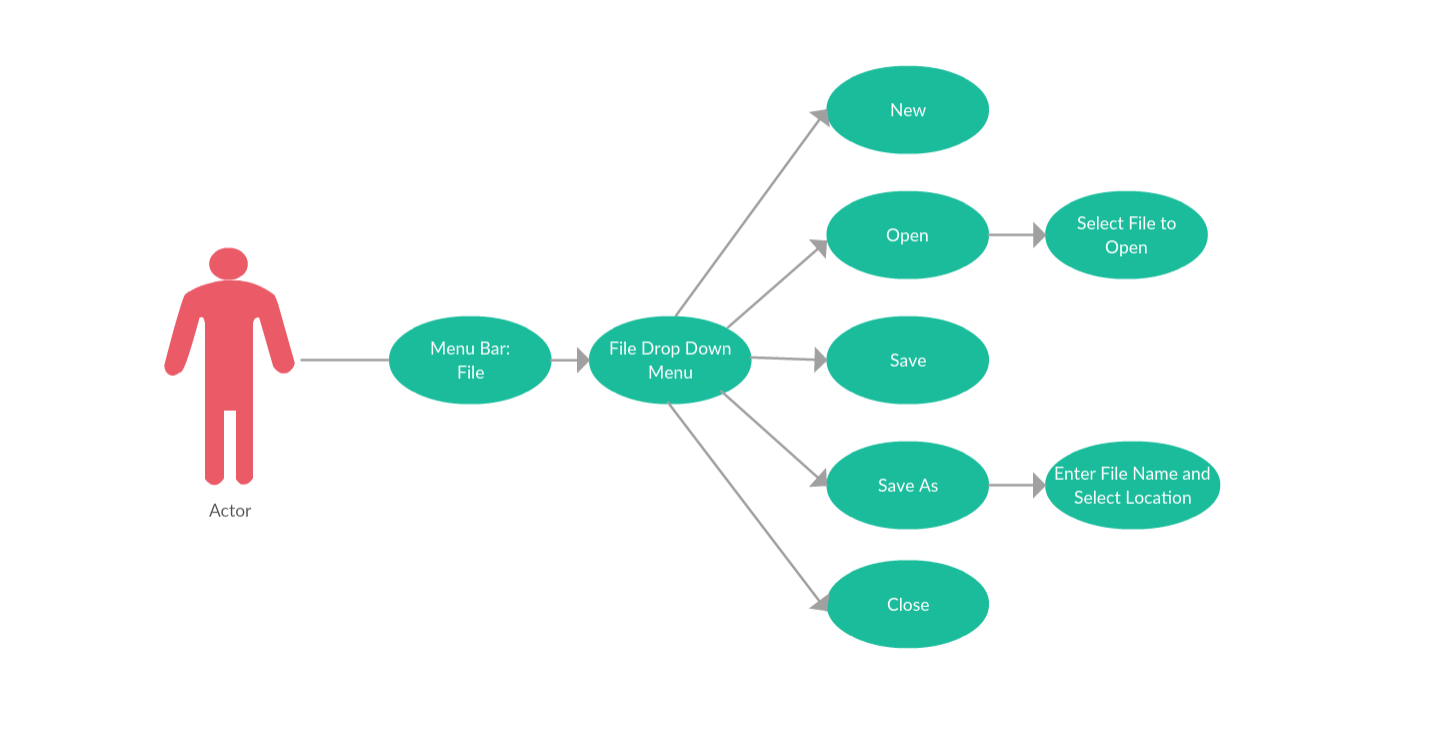
\includegraphics[width=350pt]{../UML/UseCase1.png}}
	\caption{File manipulation}
	\label{fig:UC1}
\end{figure}
\begin{figure}[H]
	\centering
	\fbox{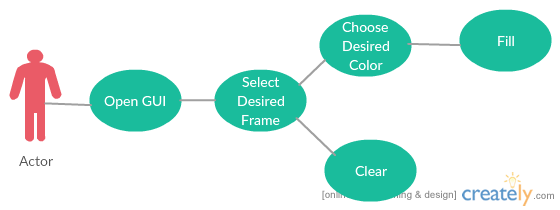
\includegraphics[width=350pt]{../UML/UseCase2.png}}
	\caption{Fill or clear frame with current color}
	\label{fig:UC2}
\end{figure}
\begin{figure}[H]
	\centering
	\fbox{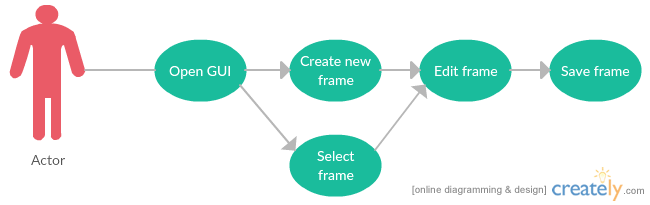
\includegraphics[width=350pt]{../UML/UseCase3.png}}
	\caption{Save/copy current frame for re-use in animation}
	\label{fig:UC3}
\end{figure}

\begin{figure}[H]
	\centering
	\fbox{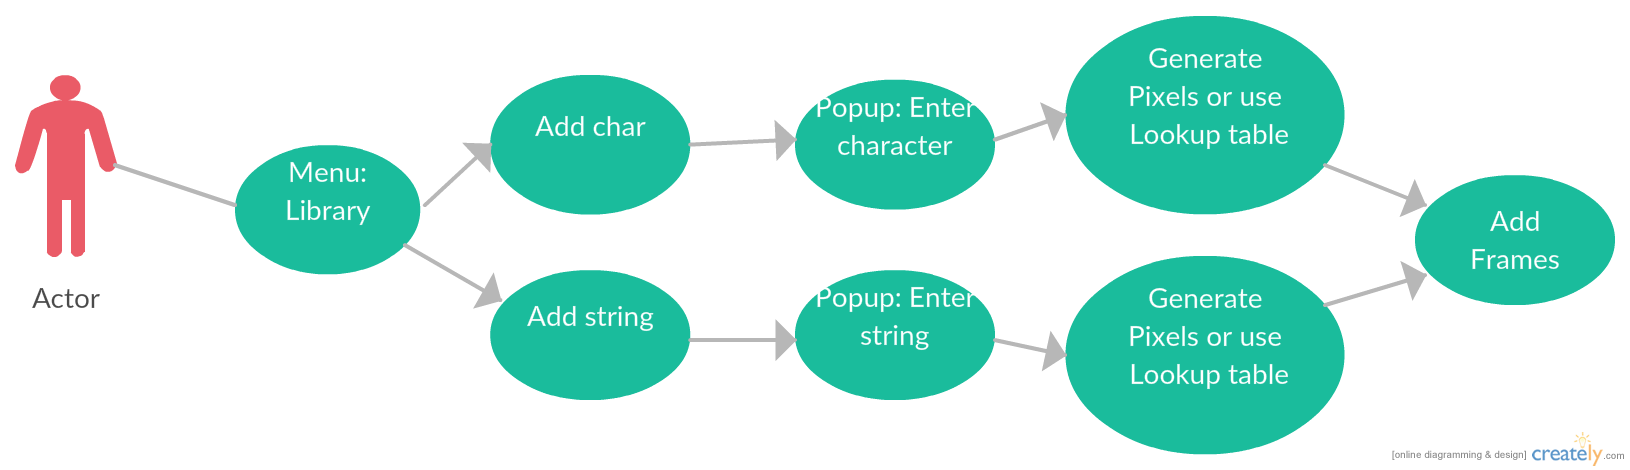
\includegraphics[width=350pt]{../UML/UseCase4.png}}
	\caption{Add char/string from predefined set}
	\label{fig:UC4}
\end{figure}

\begin{figure}[H]
	\centering
	\fbox{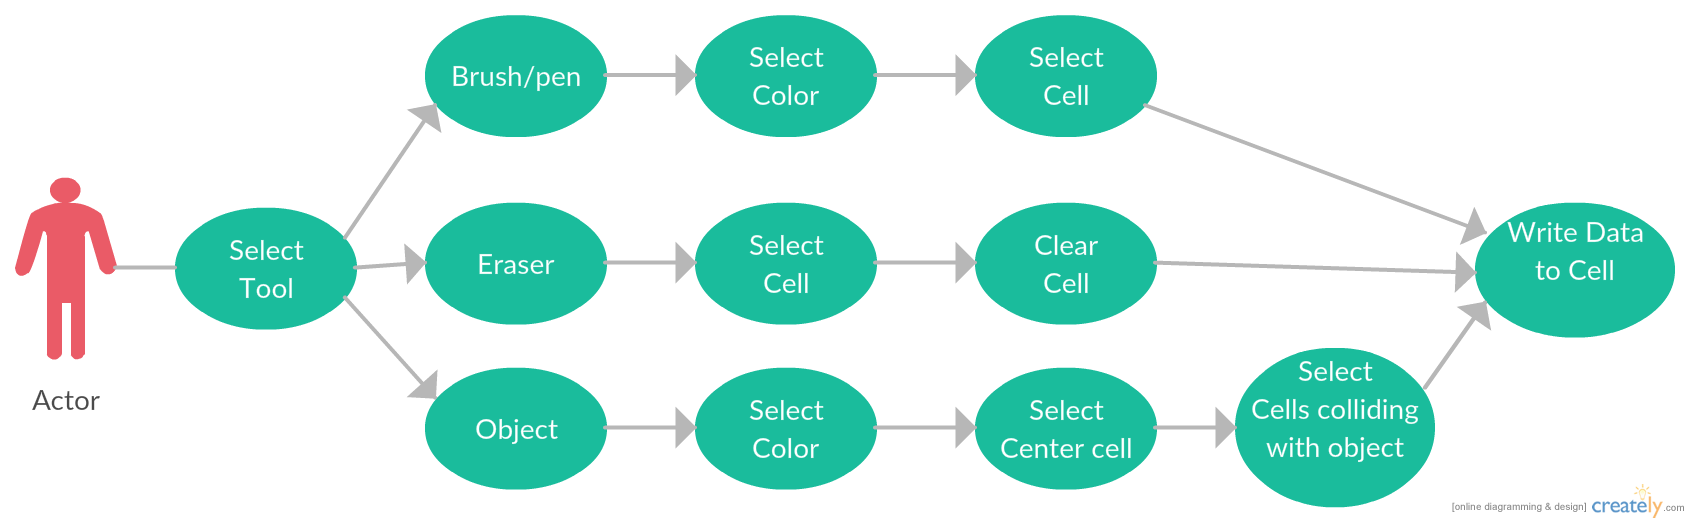
\includegraphics[width=350pt]{../UML/UseCase5.png}}
	\caption{Add a pixel in any position in any color}
	\label{fig:UC5}
\end{figure}

\begin{figure}[H]
	\centering
	\fbox{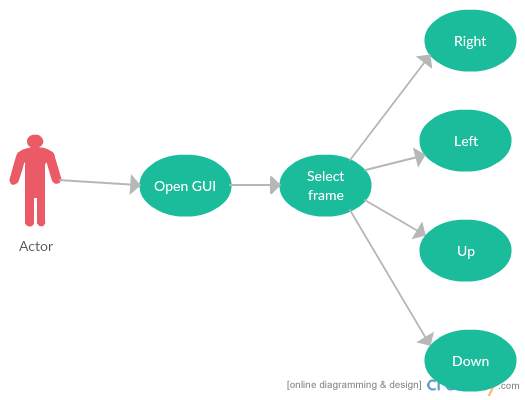
\includegraphics[width=350pt]{../UML/UseCase6.png}}
	\caption{Move everything in frame 1 pixel in a direction}
	\label{fig:UC6}
\end{figure}

\begin{figure}[H]
	\centering
	\fbox{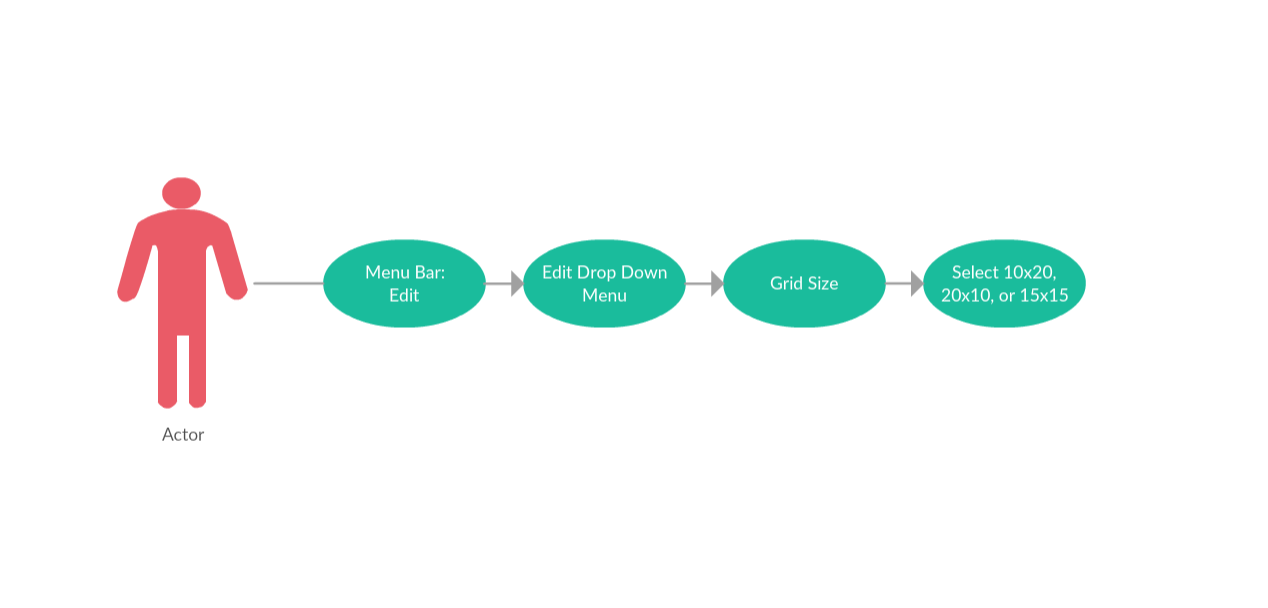
\includegraphics[width=350pt]{../UML/UseCase7.png}}
	\caption{Choose grid size for the file}
	\label{fig:UC7}
\end{figure}

\begin{figure}[H]
	\centering
	\fbox{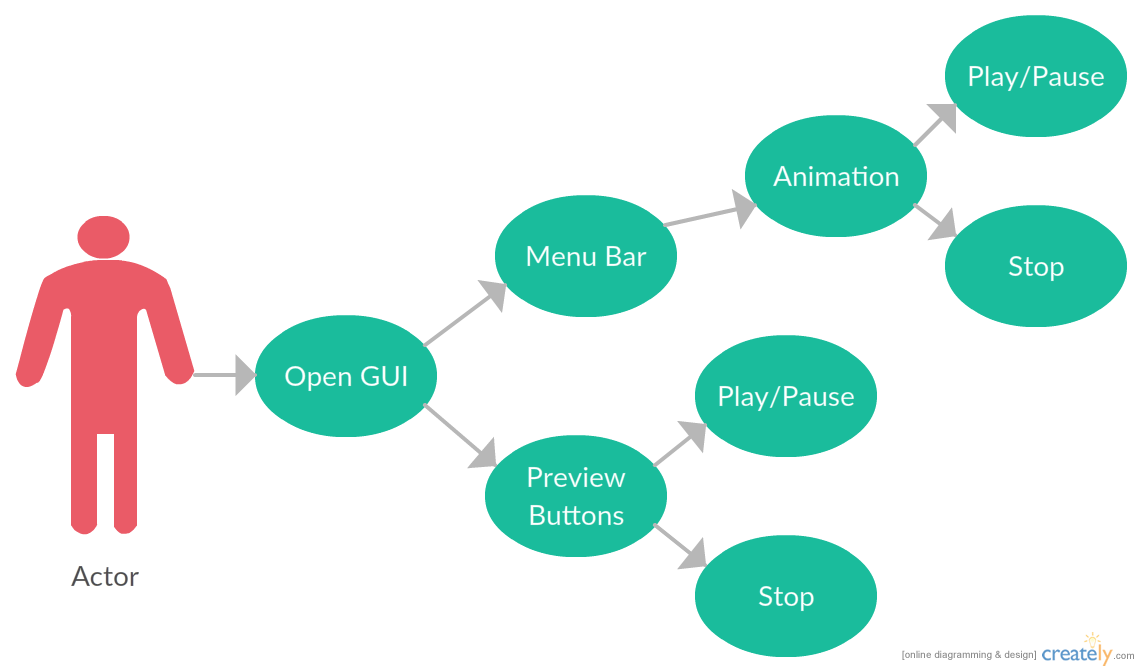
\includegraphics[width=350pt]{../UML/UseCase8.png}}
	\caption{Preview play/pause/stop animation}
	\label{fig:UC8}
\end{figure}

\begin{figure}[H]
	\centering
	\fbox{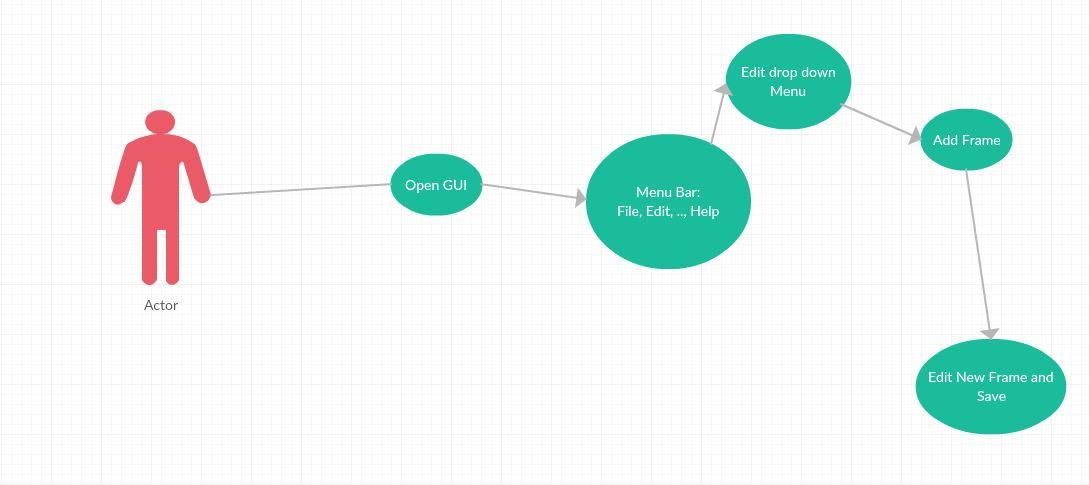
\includegraphics[width=350pt]{../UML/Create_New_Frame.jpg}}
	\caption{Create new frame}
	\label{fig:UC9}
\end{figure}

\begin{figure}[H]
	\centering
	\fbox{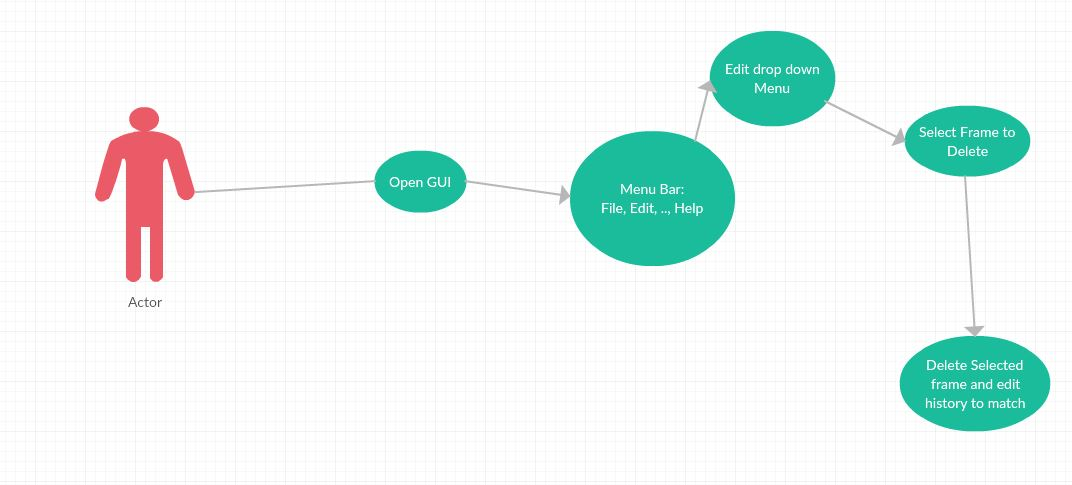
\includegraphics[width=350pt]{../UML/Delete_Frame.jpg}}
	\caption{Delete a frame}
	\label{fig:UC10}
\end{figure}

\begin{figure}[H]
	\centering
	\fbox{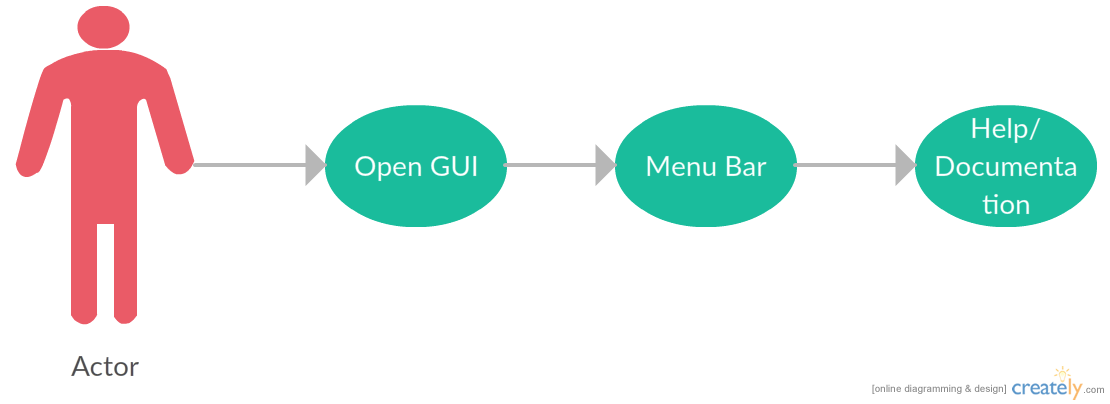
\includegraphics[width=350pt]{../UML/UseCase11.png}}
	\caption{Open help/documentation text}
	\label{fig:UC11}
\end{figure}

\begin{figure}[H]
	\centering
	\fbox{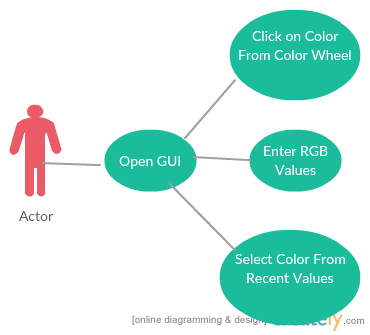
\includegraphics[width=300pt]{../UML/UseCase12.png}}
	\caption{Chose a color on the colorwheel}
	\label{fig:UC12}
\end{figure}

\begin{figure}[H]
	\centering
	\fbox{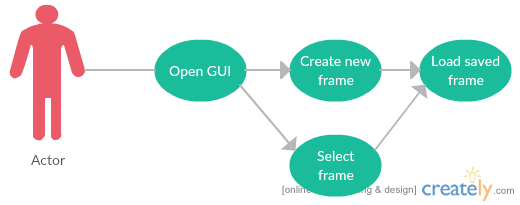
\includegraphics[width=350pt]{../UML/UseCase13.png}}
	\caption{Insert a saved frame}
	\label{fig:UC13}
\end{figure}

\begin{figure}[H]
	\centering
	\fbox{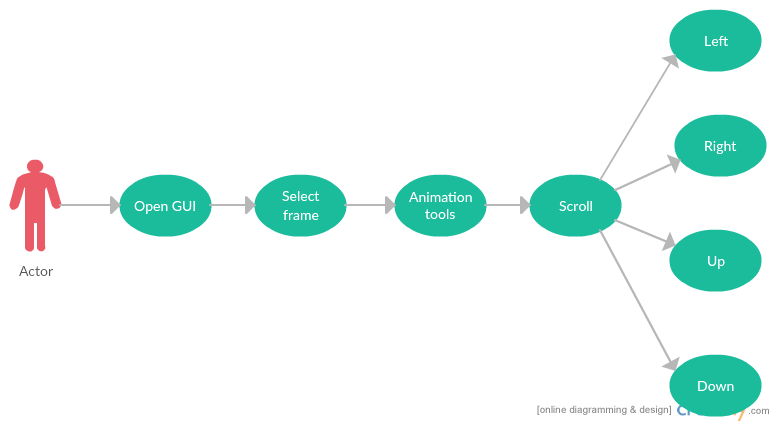
\includegraphics[width=350pt]{../UML/UseCase14.png}}
	\caption{Scroll everything across entire frame}
	\label{fig:UC14}
\end{figure}

  
\end{document}
